\chapter{Produit scalaire}

\section{Définition et propriétés}

\subsection{Norme d'un vecteur et produit scalaire}

\begin{defin}
	Soit deux points $A$ et $B$.

	La \textbf{norme} du vecteur $\vec{AB}$, notée $\norm{\vec{AB}}$, est la distance $AB$.
\end{defin}

\begin{defin}
	Soit $\vec{AB}$ et $\vec{AC}$ deux vecteurs non nuls.

	On appelle \textbf{produit scalaire} de $\vec{AB}$ par $\vec{AC}$, noté $\vec{AB}\cdot\vec{AC}$, le nombre réel défini par :
	\[
		\vec{AB}\cdot\vec{AC} = \norm{\vec{AB}} \times \norm{\vec{AC}} \times \cos\pa{\widehat{BAC}}
	\]

	Si l'un des deux vecteurs est nul, leur produit scalaire est égal à $0$.

	\begin{center}
		\begin{tikzpicture}[scale=0.9]
			\coordinate (A) at (0,0);
			\coordinate (B) at (4.5,0);
			\coordinate (C) at (2.5,2.5);
			\draw[->,very thick,rouge] (A) -- (B) node[midway,below] {$\vec{AB}$};
			\draw[->,very thick,bleu] (A) -- (C) node[midway,above left] {$\vec{AC}$};
			\draw[->] (1,0) arc[start angle=0,end angle=45,radius=1];
			\node at (22.5:1.5) {$\widehat{BAC}$};
			\node[below left] at (A) {$A$};
			\node[below right] at (B) {$B$};
			\node[above right] at (C) {$C$};
			\foreach \pt in {A, B, C}{
					\filldraw (\pt) circle (2pt);
				}
		\end{tikzpicture}
	\end{center}
\end{defin}

\begin{ex}[Calcul d'un produit scalaire avec l'angle]
	Soit $ABC$ un triangle tel que $AB = 5$, $AC = 4$ et $\widehat{BAC} = 60^\circ$ (soit $\frac{\pi}{3}$ rad).

	\begin{center}
		\begin{tikzpicture}[scale=0.8, >=Stealth]
			\coordinate (A) at (0,0);
			\coordinate (B) at (5,0);
			\coordinate (C) at (60:4);
			\draw[->, very thick, rouge] (A) -- (B) node[midway, below] {$\vec{AB}$};
			\draw[->, very thick, bleu] (A) -- (C) node[midway, above left] {$\vec{AC}$};
			\draw (C) -- (B);
			\draw[->] (0.8,0) arc[start angle=0, end angle=60, radius=0.8];
			\node at (30:1.2) {$60^\circ$};
			\node[below left] at (A) {$A$};
			\node[below right] at (B) {$B$};
			\node[above] at (C) {$C$};
			\foreach \pt in {A, B, C}{
					\filldraw (\pt) circle (2pt);
				}
		\end{tikzpicture}
	\end{center}

	Le produit scalaire des vecteurs $\vec{AB}$ et $\vec{AC}$ est égal à :
	\[
		\def\arraystretch{1.5}
		\begin{array}{rccccccl}
			\vec{AB} \cdot \vec{AC} & = & \norm{\vec{AB}} & \times & \norm{\vec{AC}} & \times & \cos\pa{\widehat{BAC}} &      \\
			                        & = & AB              & \times & AC              & \times & \cos(60^\circ)         &      \\
			                        & = & 5               & \times & 4               & \times & \dfrac{1}{2}           & = 10
		\end{array}
	\]
\end{ex}
\begin{rem}
	\nline
	\begin{itemize}
		\item $\vec{u}\cdot\vec{v}$ se lit \og $\vec{u}$ scalaire $\vec{v}$\fg{}.
		\item Le signe du produit scalaire de deux vecteurs non nuls est celui du cosinus de l'angle qu'ils forment : positif si l'angle est aigu, négatif s'il est obtus, nul s'il est droit.
	\end{itemize}
\end{rem}

\begin{attention}
	Le produit scalaire de deux vecteurs est un \textbf{nombre réel}.

	Écrire par exemple $\vec{u}\cdot\vec{v} = \vec{0}$ est une maladresse à éviter !
\end{attention}

\begin{prop}
	Pour tous points $A$ et $B$ :
	\[
		\vec{AB}\cdot\vec{AB} = \vec{AB}^2 = \norm{\vec{AB}}^2 = AB^2
	\]
\end{prop}

\begin{demo}
	L'angle $\widehat{BAB}$ est nul et $\cos 0 = 1$, donc $\vec{AB}\cdot\vec{AB} = AB \times AB \times 1 = AB^2$. Cette égalité reste vraie si $A = B$.
\end{demo}

\begin{methode}[Calculer un produit scalaire à l'aide de la formule du cosinus]
	Soit un triangle équilatéral $ABC$ de côté $5$.
	\begin{enumerate}
		\item Calculer le produit scalaire $\vec{AB}\cdot\vec{AC}$.
		\item Soit $I$ le milieu de $[AB]$. Calculer le produit scalaire $\vec{AI}\cdot\vec{BC}$.
	\end{enumerate}

	\begin{center}
		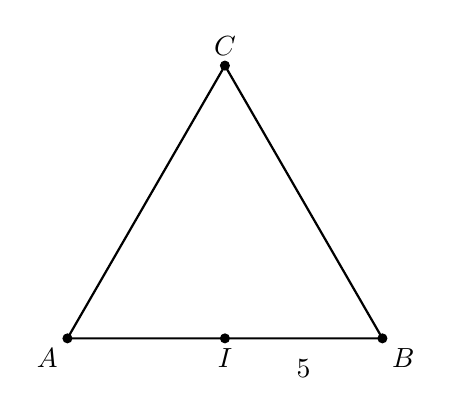
\begin{tikzpicture}[scale=0.8]
			\coordinate (A) at (0,0);
			\coordinate (B) at (5,0);
			\coordinate (C) at (2.5,{5*sin(60)});
			\coordinate (I) at (2.5,0);
			\draw[thick] (A) -- (B) -- (C) -- cycle;
			\node[below left] at (A) {$A$};
			\node[below right] at (B) {$B$};
			\node[above] at (C) {$C$};
			\node[below] at (I) {$I$};
			\node[below=4pt] at (3.75,0) {$5$};
			\foreach \pt in {A, B, C, I}{
					\filldraw (\pt) circle (2pt);
				}
		\end{tikzpicture}
	\end{center}

	\begin{correction}
		\nline
		\begin{enumerate}
			\item Le triangle $ABC$ est équilatéral : $\widehat{BAC} = 60^\circ = \frac{\pi}{3}$ et $AB = AC = 5$.
			      \[
				      \begin{array}{rccccccl}
					      \vec{AB}\cdot\vec{AC} & = AB & \times & AC & \times & \cos\pa{\widehat{BAC}} &          \\
					                            & = 5  & \times & 5  & \times & \cos 60^\circ          &          \\
					                            & = 25 &        &    & \times & 0{,}5                  & = 12{,}5
				      \end{array}
			      \]

			\item Les vecteurs $\vec{AI}$ et $\vec{BC}$ n'ont pas la même origine. On construit le point $D$ tel que $\vec{AD} = \vec{BC}$ : le produit scalaire à calculer est alors composé de deux vecteurs de même origine $A$.

			      \begin{center}
				      \begin{tikzpicture}[scale=0.8]
					      \coordinate (A) at (0,0);
					      \coordinate (B) at (5,0);
					      \coordinate (C) at (2.5,{5*sin(60)});
					      \coordinate (I) at (2.5,0);
					      \coordinate (D) at (-2.5,{5*sin(60)});
					      \draw[thick] (A) -- (B) -- (C) -- cycle;
					      \draw[->,ultra thick,vert,dashed] (B) -- (C) node[midway,sloped, above] {$\vec{BC}$};
					      \draw[->,ultra thick,rouge] (A) -- (D) node[midway,sloped, above] {$\vec{BC}$};
					      \draw[->,ultra thick,rouge] (A) -- (I) node[midway,below] {$\vec{AI}$};
					      \draw[->] (0.8,0) arc[start angle=0,end angle=120,radius=0.8];
					      \node[fill=white,inner sep=1pt] at (90:1.25) {$\frac{2\pi}{3}$};
					      \fill (I) circle (1.5pt);
					      \node[below left] at (A) {$A$};
					      \node[below right] at (B) {$B$};
					      \node[above right] at (C) {$C$};
					      \node[above left] at (D) {$D$};
					      \node[below right] at (I) {$I$};
					      \foreach \pt in {A, B, C, D, I}{
							      \filldraw (\pt) circle (2pt);
						      }
				      \end{tikzpicture}
			      \end{center}

			      Comme $I$ est le milieu de $[AB]$, $AI = 2{,}5$ ; de plus $AD = BC = 5$ et $\widehat{IAD} = \frac{2\pi}{3}$.
			      \[
				      \begin{array}{rccccccl}
					      \vec{AI}\cdot\vec{BC} & = & \vec{AI} & \cdot  & \vec{AD} &        &                        &           \\
					                            & = & AI       & \times & AD       & \times & \cos\pa{\widehat{IAD}} &           \\
					                            & = & 2{,}5    & \times & 5        & \times & \cos\frac{2\pi}{3}     &           \\
					                            & = & 12{,}5   &        &          & \times & \pa{-0{,}5}            & = -6{,}25
				      \end{array}
			      \]
		\end{enumerate}
	\end{correction}
\end{methode}

\subsection{Propriétés du produit scalaire}

\begin{prop}[Symétrie]
	Pour tous vecteurs $\vec{u}$ et $\vec{v}$ :
	\[
		\vec{u}\cdot\vec{v} = \vec{v}\cdot\vec{u}
	\]
\end{prop}

\begin{demo}
	\begin{demo}
		Soient $\vec{u}$ et $\vec{v}$ deux vecteurs non nuls.

		On sait que les angles orientés vérifient $(\vec{v},\vec{u}) = -(\vec{u},\vec{v})$.

		Par parité de la fonction cosinus, pour tout réel $x$, $\cos(-x) = \cos(x)$.

		On a donc :
		\[
			\begin{array}{rcl}
				\cos\pa{(\vec{v},\vec{u})} & = & \cos\pa{-(\vec{u},\vec{v})} \\
				                           & = & \cos\pa{(\vec{u},\vec{v})}
			\end{array}
		\]

		D'où :
		\[
			\begin{array}{rccccccl}
				\vec{v}\cdot\vec{u} & = & \norm{\vec{v}} & \times & \norm{\vec{u}} & \times & \cos\pa{(\vec{v},\vec{u})} &                       \\
				                    & = & \norm{\vec{u}} & \times & \norm{\vec{v}} & \times & \cos\pa{(\vec{u},\vec{v})} & = \vec{u}\cdot\vec{v}
			\end{array}
		\]

		Si l'un des vecteurs est nul, le produit scalaire vaut $0$ dans les deux cas, ce qui confirme l'égalité.
	\end{demo}
\end{demo}

\begin{prop}[Bilinéarité (admise)]
	Pour tous vecteurs $\vec{u}$, $\vec{v}$, $\vec{w}$ et tout réel $k$ :
	\begin{multicols}{2}
		\begin{enumerate}
			\item $\vec{u}\cdot\pa{\vec{v} + \vec{w}} = \vec{u}\cdot\vec{v} + \vec{u}\cdot\vec{w}$
			\item $\vec{u}\cdot\pa{k\vec{v}} = k\,\vec{u}\cdot\vec{v}$
		\end{enumerate}
	\end{multicols}

	Grâce à la symétrie, on a de même $\pa{\vec{u} + \vec{v}}\cdot\vec{w} = \vec{u}\cdot\vec{w} + \vec{v}\cdot\vec{w}$ et $\pa{k\vec{u}}\cdot\vec{v} = k\,\vec{u}\cdot\vec{v}$.
\end{prop}

\begin{prop}[Identités remarquables]
	Pour tous vecteurs $\vec{u}$ et $\vec{v}$ :
	\begin{enumerate}
		\item $\pa{\vec{u} + \vec{v}}^2 = \vec{u}^2 + 2\,\vec{u}\cdot\vec{v} + \vec{v}^2$ \quad soit \quad $\norm{\vec{u} + \vec{v}}^2 = \norm{\vec{u}}^2 + 2\,\vec{u}\cdot\vec{v} + \norm{\vec{v}}^2$ ;
		\item $\pa{\vec{u} - \vec{v}}^2 = \vec{u}^2 - 2\,\vec{u}\cdot\vec{v} + \vec{v}^2$ \quad soit \quad $\norm{\vec{u} - \vec{v}}^2 = \norm{\vec{u}}^2 - 2\,\vec{u}\cdot\vec{v} + \norm{\vec{v}}^2$ ;
		\item $\pa{\vec{u} + \vec{v}}\cdot\pa{\vec{u} - \vec{v}} = \vec{u}^2 - \vec{v}^2$ \quad soit \quad $\pa{\vec{u} + \vec{v}}\cdot\pa{\vec{u} - \vec{v}} = \norm{\vec{u}}^2 - \norm{\vec{v}}^2$.
	\end{enumerate}
\end{prop}

\begin{demo}
	On utilise la bilinéarité, la symétrie et le fait que $\vec{w}\cdot\vec{w} = \vec{w}^2 = \norm{\vec{w}}^2$ :
	\begin{enumerate}
		\item $\pa{\vec{u} + \vec{v}}\cdot\pa{\vec{u} + \vec{v}} = \pa{\vec{u}\cdot\vec{u}} + \pa{\vec{u}\cdot\vec{v}} + \pa{\vec{v}\cdot\vec{u}} + \pa{\vec{v}\cdot\vec{v}} = \vec{u}^2 + 2\,\vec{u}\cdot\vec{v} + \vec{v}^2$ ;
		\item $\pa{\vec{u} - \vec{v}}\cdot\pa{\vec{u} - \vec{v}} = \pa{\vec{u}\cdot\vec{u}} - \pa{\vec{u}\cdot\vec{v}} - \pa{\vec{v}\cdot\vec{u}} + \pa{\vec{v}\cdot\vec{v}} = \vec{u}^2 - 2\,\vec{u}\cdot\vec{v} + \vec{v}^2$ ;
		\item $\pa{\vec{u} + \vec{v}}\cdot\pa{\vec{u} - \vec{v}} = \pa{\vec{u}\cdot\vec{u}} - \pa{\vec{u}\cdot\vec{v}} + \pa{\vec{v}\cdot\vec{u}} - \pa{\vec{v}\cdot\vec{v}} = \vec{u}^2 - \vec{v}^2$.
	\end{enumerate}
\end{demo}

\begin{methode}[Appliquer les propriétés du produit scalaire]
	Soit $\vec{u}$ et $\vec{v}$ deux vecteurs de normes respectives $2$ et $3$ et tels que $\vec{u}\cdot\vec{v} = 1$. Calculer :

	\begin{enumerate}
		\item $\pa{\vec{u} + \vec{v}}\cdot\pa{\vec{u} - \vec{v}}$ ;
		\item $\vec{u}\cdot\pa{\vec{u} + \vec{v}}$ ;
		\item $-2\vec{v}\cdot\pa{3\vec{u} - \vec{v}}$.
	\end{enumerate}

	\begin{correction}
		\nline
		\begin{enumerate}
			\item $\pa{\vec{u} + \vec{v}}\cdot\pa{\vec{u} - \vec{v}} = \norm{\vec{u}}^2 - \norm{\vec{v}}^2 = 2^2 - 3^2 = -5$.
			\item $\vec{u}\cdot\pa{\vec{u} + \vec{v}} = \pa{\vec{u}\cdot\vec{u}} + \pa{\vec{u}\cdot\vec{v}} = \norm{\vec{u}}^2 + \vec{u}\cdot\vec{v} = 2^2 + 1 = 5$.
			\item $-2\vec{v}\cdot\pa{3\vec{u} - \vec{v}} = \pa{-6\,\vec{v}\cdot\vec{u}} + \pa{2\,\vec{v}\cdot\vec{v}} = -6\,\vec{u}\cdot\vec{v} + 2\norm{\vec{v}}^2 = -6 \times 1 + 2 \times 3^2 = 12$.
		\end{enumerate}
	\end{correction}
\end{methode}

\subsection{Une autre expression du produit scalaire}

\begin{prop}
	Pour tous vecteurs $\vec{u}$ et $\vec{v}$ :
	\[
		\vec{u}\cdot\vec{v} = \dfrac{1}{2}\pa{\norm{\vec{u} + \vec{v}}^2 - \norm{\vec{u}}^2 - \norm{\vec{v}}^2}
		\qquad\text{et}\qquad
		\vec{u}\cdot\vec{v} = \dfrac{1}{2}\pa{\norm{\vec{u}}^2 + \norm{\vec{v}}^2 - \norm{\vec{u} - \vec{v}}^2}
	\]

\end{prop}
\begin{demo}
	\nline
	\begin{itemize}
		\item \textbf{Pour la première égalité :}

		      Soient $\vec{u}$ et $\vec{v}$ deux vecteurs.

		      En utilisant l'identité remarquable vectorielle $(\vec{u} + \vec{v})^2$, on a :
		      \[
			      \begin{array}{rcccl}
				      (\vec{u} + \vec{v})^2 & = & \norm{\vec{u} + \vec{v}}^2 & = & (\vec{u} + \vec{v}) \cdot (\vec{u} + \vec{v})                          \\[2mm]
				                            &   &                            & = & \vec{u} \cdot \vec{u} + 2\,\vec{u}\cdot\vec{v} + \vec{v} \cdot \vec{v} \\[2mm]
				                            &   &                            & = & \norm{\vec{u}}^2 + 2\,\vec{u}\cdot\vec{v} + \norm{\vec{v}}^2
			      \end{array}
		      \]
		      En isolant le terme $2\,\vec{u}\cdot\vec{v}$, on obtient :
		      \[
			      2\,\vec{u}\cdot\vec{v} = \norm{\vec{u} + \vec{v}}^2 - \norm{\vec{u}}^2 - \norm{\vec{v}}^2
		      \]
		      Puis, en divisant par $2$, on retrouve bien :
		      \[
			      \vec{u}\cdot\vec{v} = \dfrac{1}{2}\pa{\norm{\vec{u} + \vec{v}}^2 - \norm{\vec{u}}^2 - \norm{\vec{v}}^2}
		      \]

		\item \textbf{Pour la seconde égalité :}

		      On procède de manière analogue en développant $(\vec{u} - \vec{v})^2$.
	\end{itemize}
\end{demo}

\begin{ex}
	Soit $ABCD$ un parallélogramme tel que $AB = 4$, $AD = 3$ et $AC = 6$.

	\begin{center}
		\begin{tikzpicture}
			\coordinate (A) at (0,0);
			\coordinate (B) at (4,0);
			\coordinate (D) at (1.375,{sqrt(9-1.375*1.375)});
			\coordinate (C) at (5.375,{sqrt(9-1.375*1.375)});
			\draw[thick] (A) -- (B) -- (C) -- (D) -- cycle;
			\draw[dashed,gris] (A) -- (C) node[sloped, midway, above] {$6$};
			\draw[dashed,gris] (A) -- (D) node[sloped, midway, below] {$3$};
			\draw[dashed,gris] (A) -- (B) node[sloped, midway, above] {$4$};
			\node[below left] at (A) {$A$};
			\node[below right] at (B) {$B$};
			\node[above right] at (C) {$C$};
			\node[above left] at (D) {$D$};
			\draw[->,very thick,rouge] (A) -- (D) node[sloped, midway, above] {$\vec{AD}$};
			\draw[->,very thick,rouge] (A) -- (B) node[sloped, midway, below] {$\vec{AB}$};
			\draw[->,very thick,bleu] (A) -- (C) node[sloped, midway, below] {$\vec{AC}$};
			\foreach \pt in {A, B, C, D}{
					\filldraw (\pt) circle (2pt);
				}
		\end{tikzpicture}
	\end{center}

	On a :
	\[
		\vec{AB}\cdot\vec{AD} = \dfrac{1}{2}\pa{\norm{\vec{AB} + \vec{AD}}^2 - \norm{\vec{AB}}^2 - \norm{\vec{AD}}^2}
	\]

	Comme $\vec{AB} + \vec{AD} = \vec{AC}$, on obtient :
	\[
		\begin{array}{rcll}
			\vec{AB}\cdot\vec{AD} & = & \frac{1}{2}\pa{\norm{\vec{AB} + \vec{AD}}^2 - \norm{\vec{AB}}^2 - \norm{\vec{AD}}^2} &                 \\
			                      & = & \frac{1}{2}\pa{AC^2 - AB^2 - AD^2}                                                                     \\
			                      & = & \frac{1}{2}\pa{36 - 16 - 9}                                                          & = \dfrac{11}{2}
		\end{array}
	\]

\end{ex}

\section{Produit scalaire et orthogonalité}

\subsection{Vecteurs orthogonaux}

\begin{prop}
	Les vecteurs $\vec{u}$ et $\vec{v}$ sont orthogonaux si et seulement si $\vec{u}\cdot\vec{v} = 0$.

	\[
		\vec{u} \perp \vec{v} \iff \vec{u}\cdot\vec{v}=0
	\]
\end{prop}

\begin{demo}
	Si l'un des vecteurs est nul, le résultat est immédiat (le vecteur nul est orthogonal à tout vecteur et le produit scalaire est nul).

	Supposons les deux vecteurs non nuls et notons $\vec{u} = \vec{AB}$ et $\vec{v} = \vec{AC}$. On a :
	\[
		\def\arraystretch{1.3}
		\begin{array}{rcccl}
			\vec{u}\cdot\vec{v} = 0 & \eqv & AB \times AC \times & \cos\pa{\widehat{BAC}} = 0 &                               \\
			                        & \eqv &                     & \cos\pa{\widehat{BAC}} = 0 & \eqv \widehat{BAC} = 90^\circ
		\end{array}
	\]

	\ldots car $AB \neq 0$ et $AC \neq 0$.

	Les vecteurs $\vec{u}$ et $\vec{v}$ sont donc orthogonaux.
\end{demo}

\begin{rem}
	Deux droites $(AB)$ et $(CD)$ sont perpendiculaires si et seulement si les vecteurs $\vec{AB}$ et $\vec{CD}$ sont orthogonaux, c'est-à-dire si et seulement si $\vec{AB}\cdot\vec{CD} = 0$.
\end{rem}

\subsection{Projeté orthogonal}

\begin{defin}
	Soit une droite $d$ et un point $M$.

	Le \textbf{projeté orthogonal} du point $M$ sur la droite $d$ est le point d'intersection $H$ de la droite $d$ avec la perpendiculaire à $d$ passant par $M$.
	\begin{center}
		\begin{tikzpicture}[scale=0.9, >=Stealth]
			\draw[thick, gris,domain=0:4.5] plot (\x , 0.5*\x) node[fill=white, right] {$\pa{d}$};
			\draw[thick, dashed, rouge, domain=1:2] plot (\x , -2*\x+5);
			\coordinate (M) at (1, 3);
			\coordinate (H) at (2, 1);
			\draw[thick, rouge] ($(H)!0.3cm!(M)$) -- ($(H)!0.3cm!(M) + ($(H)!0.3cm!(-1,-0.5)$)-(H)$) -- ($(H)!0.3cm!(-1,-0.5)$);
			\fill[bleu] (M) circle (2.5pt) node[left] {$M$};
			\fill[rouge] (H) circle (2.5pt) node[below right] {$H$};
		\end{tikzpicture}
	\end{center}\end{defin}

\begin{prop}
	Soit $\vec{OA}$ et $\vec{OB}$ deux vecteurs non nuls et $H$ le projeté orthogonal du point $B$ sur la droite $(OA)$. Alors :
	\[
		\vec{OA}\cdot\vec{OB} = \vec{OA}\cdot\vec{OH}
	\]
\end{prop}

\begin{demo}
	\nline
	\begin{wrapstuff}[r]
		\begin{tikzpicture}[scale=0.9]
			\coordinate (O) at (0,0);
			\coordinate (A) at (5,0);
			\coordinate (B) at (3.6,2.5);
			\coordinate (H) at (3.6,0);
			\draw[->, very thick, bleu] (O) -- (A);
			\draw[->, very thick, bleu] (O) -- (B);
			\draw[->, very thick, rouge] (O) -- (H);
			\draw[dashed] (B) -- (H);
			\draw (3.35,0) -- (3.35,0.25) -- (3.6,0.25);
			\node[below left] at (O) {$O$};
			\node[right] at (A) {$A$};
			\node[above right] at (B) {$B$};
			\node[below] at (H) {$H$};
		\end{tikzpicture}
	\end{wrapstuff}

	D'après la relation de Chasles, $\vec{OB} = \vec{OH} + \vec{HB}$, donc
	\[
		\def\arraystretch{1.3}
		\begin{array}{rcll}
			\vec{OA}\cdot\vec{OB} & = & \vec{OA}\cdot\pa{\vec{OH} + \vec{HB}}                           &                         \\
			                      & = & \vec{OA}\cdot\vec{OH} + \underbrace{\vec{OA}\cdot\vec{HB}}_{=0} & = \vec{OA}\cdot\vec{OH}
		\end{array}
	\]

	En effet, les vecteurs $\vec{OA}$ et $\vec{HB}$ sont orthogonaux donc $\vec{OA}\cdot\vec{HB} = 0$.
\end{demo}

\newpage

\begin{rem}
	Cette propriété permet de simplifier considérablement le calcul du produit scalaire : en remplaçant le vecteur $\vec{OB}$ par son projeté orthogonal $\vec{OH}$ sur la droite $(OA)$, on se ramène au produit scalaire de deux vecteurs colinéaires.

	Le calcul se réduit alors à un simple produit de longueurs, précédé d'un signe $+$ si $\vec{OA}$ et $\vec{OH}$ sont de même sens, ou d'un signe $-$ s'ils sont de sens contraires.
\end{rem}

\begin{methode}[Calculer un produit scalaire par projection]
	Soit un carré $ABCD$ de côté $4$.

	\begin{center}
		\begin{tikzpicture}[scale=0.6]
			\coordinate (A) at (0,0);
			\coordinate (B) at (4,0);
			\coordinate (C) at (4,4);
			\coordinate (D) at (0,4);
			\draw[thick] (A) -- (B) -- (C) -- (D) -- cycle;
			\draw[gris] (A) -- (C);
			\foreach \pa/\pb/\c in {A/B/rouge, A/C/bleu, A/D/vert, C/B/orange}{
					\draw[very thick, ->,\c] (\pa) -- (\pb);
				}
			\node[below left] at (A) {$A$};
			\node[below right] at (B) {$B$};
			\node[above right] at (C) {$C$};
			\node[above left] at (D) {$D$};
			\node[above] at (2,4) {$4$};

			\foreach \pt in {A, B, C, D}{
					\filldraw (\pt) circle (3pt);
				}
		\end{tikzpicture}
	\end{center}

	Calculer les produits scalaires :

	\begin{multicols}{3}
		\begin{enumerate}
			\item $\vec{AB}\cdot\vec{AC}$ ;
			\item $\vec{AB}\cdot\vec{AD}$ ;
			\item $\vec{AD}\cdot\vec{CB}$.
		\end{enumerate}
	\end{multicols}

	\begin{correction}
		\nline
		\begin{enumerate}
			\item $B$ est le projeté orthogonal de $C$ sur $(AB)$, donc :
			      \[
				      \begin{array}{rccccl}
					      \vec{AB}\cdot\vec{AC} & = & \vec{AB}        & \cdot  & \vec{AB}        &                   \\
					                            & = & \norm{\vec{AB}} & \times & \norm{\vec{AB}} & = AB^2 = 4^2 = 16
				      \end{array}
			      \]

			\item $\vec{AB}\cdot\vec{AD} = 0$ car les vecteurs $\vec{AB}$ et $\vec{AD}$ sont orthogonaux.
			\item Comme $\vec{CB} = \vec{DA}$, on a :
			      \[
				      \begin{array}{rccl}
					      \vec{AD}\cdot\vec{CB} & = & \vec{AD}\cdot\vec{DA}  &                                         \\
					                            & = & -\vec{AD}\cdot\vec{AD} & =-\norm{\vec{AD}}^2= -AD^2 = -4^2 = -16
				      \end{array}
			      \]

		\end{enumerate}
	\end{correction}
\end{methode}

\section{Produit scalaire dans un repère orthonormé}

Dans toute cette partie, le plan est muni d'un repère orthonormé $\vOIJ$.

\begin{prop}
	Soit $\vec{u}\coord{x}{y}$ et $\vec{v}\coord{x'}{y'}$ deux vecteurs. Alors :
	\[
		\vec{u}\cdot\vec{v} = xx' + yy' \quad\text{et}\quad \norm{\vec{u}}^2 = x^2 + y^2
	\]

\end{prop}

\begin{demo}
	\nline
	\begin{enumerate}
		\item \textbf{Norme du vecteur $\vec{u}$ :}

		      Dans un repère orthonormé, la longueur d'un vecteur $\vec{u}\coord{x}{y}$ s'obtient directement en appliquant le théorème de Pythagore (vu en seconde) :
		      \[
			      \norm{\vec{u}} = \sqrt{x^2 + y^2}
		      \]
		      En élevant cette expression au carré, on retrouve bien :
		      \[
			      \norm{\vec{u}}^2 = x^2 + y^2
		      \]

		\item \textbf{Calcul du produit scalaire $\vec{u}\cdot\vec{v}$ :}

		      Les vecteurs $\vec{u}$ et $\vec{v}$ ont pour coordonnées respectives $\coord{x}{y}$ et $\coord{x'}{y'}$.

		      Le vecteur somme $\pa{\vec{u} + \vec{v}}$ a donc pour coordonnées $\coord{x + x'}{y + y'}$.

		      Exprimons la norme au carré des trois vecteurs $\vec{u}$, $\vec{v}$ et $\pa{\vec{u} + \vec{v}}$ :
		      \begin{itemize}
			      \item $\norm{\vec{u}}^2 = x^2 + y^2$
			      \item $\norm{\vec{v}}^2 = x'^2 + y'^2$
			      \item $\norm{\vec{u} + \vec{v}}^2 = (x + x')^2 + (y + y')^2$
		      \end{itemize}

		      Utilisons la formule du produit scalaire exprimée à l'aide des normes :
		      \[
			      \def\arraystretch{1.4}
			      \begin{array}{rcl}
				      \vec{u}\cdot\vec{v} & = & \frac{1}{2}\pa{\norm{\vec{u} + \vec{v}}^2 - \norm{\vec{u}}^2 - \norm{\vec{v}}^2}   \\
				                          & = & \frac{1}{2}\bra{\pa{x + x'}^2 + \pa{y + y'}^2 - \pa{x^2 + y^2} - \pa{x'^2 + y'^2}} \\
				                          & = & \frac{1}{2}\bra{x^2 + 2xx' + x'^2 + y^2 + 2yy' + y'^2 - x^2 - y^2 - x'^2 - y'^2}   \\
				                          & = & \frac{1}{2}\bra{2xx' + 2yy'} = \frac{1}{2} \times 2 \pa{xx' + yy'}                 \\
				                          & = & xx' + yy'
			      \end{array}
		      \]
	\end{enumerate}
\end{demo}

\begin{methode}[Calculer un produit scalaire à l'aide des coordonnées]
	\nline
	\begin{enumerate}
		\item Soit $\vec{u}\coord{5}{-4}$ et $\vec{v}\coord{-3}{7}$ deux vecteurs. Calculer $\vec{u}\cdot\vec{v}$.
		\item On considère les points $A\coordl{2}{1}$, $B\coordl{5}{3}$, $C\coordl{1}{4}$ et $D\coordl{5}{-2}$. Démontrer que les droites $(AB)$ et $(CD)$ sont perpendiculaires.
	\end{enumerate}

	\begin{correction}
		\nline
		\begin{enumerate}
			\item $\vec{u}\cdot\vec{v} = 5 \times \pa{-3} + \pa{-4} \times 7 = -15 - 28 = -43$.
			\item On calcule les coordonnées des vecteurs $\vec{AB}$ et $\vec{CD}$ :
			      \[
				      \vec{AB}\coord{5 - 2}{3 - 1} = \vec{AB}\coord{3}{2} \quad\text{et}\quad \vec{CD}\coord{5 - 1}{-2 - 4} = \vec{CD}\coord{4}{-6}
			      \]

			      Puis leur produit scalaire :
			      \[
				      \vec{AB}\cdot\vec{CD} = 3 \times 4 + 2 \times \pa{-6} = 12 - 12 = 0
			      \]

			      Le produit scalaire est nul donc les vecteurs $\vec{AB}$ et $\vec{CD}$ sont orthogonaux. Les droites $(AB)$ et $(CD)$ sont donc perpendiculaires.
		\end{enumerate}
		\begin{center}
			\begin{tikzpicture}[scale=0.7, >=Stealth]
				\clip (-0.5,-3.2) rectangle (6.2,4.5);
				\draw[xstep=1, ystep=1, gray!40, dashed] (-0.5,-3.2) grid (6,5);
				\draw[->, thick] (-0.5,0) -- (6.2,0) node[below left] {$x$};
				\draw[->, thick] (0,-3.2) -- (0,4.5) node[below left] {$y$};
				\node[below left] at (0,0) {$0$};
				\coordinate (A) at (2,1);
				\coordinate (B) at (5,3);
				\coordinate (C) at (1,4);
				\coordinate (D) at (5,-2);
				\draw[dashed, domain=0:6.2, smooth, variable=\x, thick, rouge] plot ({\x}, {(2/3)*\x - 1/3});
				\draw[dashed, domain=0:6.5, smooth, variable=\x, thick, vert] plot ({\x}, {-1.5*\x + 5.5});
				\draw[->, very thick, rouge] (A) -- (B) node[sloped, midway, above] {$\vec{AB}$};
				\draw[->, very thick, vert] (C) -- (D) node[sloped, midway, above right] {$\vec{CD}$};
				\foreach \pt in {A, B, C, D}{
						\filldraw (\pt) circle (2pt);
					}
			\end{tikzpicture}
		\end{center}	\end{correction}
\end{methode}

\newpage

\begin{methode}[Appliquer plusieurs formules du produit scalaire]
	Dans le repère orthonormé ci-dessous, les droites $(AB)$ et $(CD)$ se coupent en un point $E$.

	On veut calculer la mesure de l'angle $\widehat{BED}$ en calculant le produit scalaire $\vec{AB}\cdot\vec{CD}$ de deux façons.

	On pourra lire les coordonnées des points $A$, $B$, $C$ et $D$ sur le repère.

	\begin{center}
		\begin{tikzpicture}[scale=1.3]
			\draw[gris!40,dashed] (-1.5,-1.5) grid (4.7,3.5);
			\draw[->] (-1.5,0) -- (4.7,0);
			\draw[->] (0,-1.5) -- (0,3.5);
			\foreach \i in {-1,1,2,3,4} {\node[below] at (\i,0) {$\i$};}
			\foreach \j in {-1,1,2,3} {\node[left] at (0,\j) {$\j$};}
			\node[below left] at (0,0) {$0$};
			\coordinate (A) at (-1,2);
			\coordinate (B) at (4,1);
			\coordinate (C) at (4,3);
			\coordinate (D) at (2,-1);
			\coordinate (E) at ({34/11},{13/11});
			\draw[thick,bleu] (A) -- (B);
			\draw[thick,rouge] (C) -- (D);
			\fill (A) circle (1.5pt);
			\fill (B) circle (1.5pt);
			\fill (C) circle (1.5pt);
			\fill (D) circle (1.5pt);
			\fill (E) circle (1.5pt);
			\node[above left] at (A) {$A$};
			\node[right] at (B) {$B$};
			\node[above right] at (C) {$C$};
			\node[below] at (D) {$D$};
			\node[above left] at (E) {$E$};
			\draw[->, thick] ($(E)+(-11.31:0.6)$) arc[start angle=-11.31,end angle=-116.565,radius=0.6];
		\end{tikzpicture}
	\end{center}

	\begin{correction}
		On lit $A\coordl{-1}{2}$, $B\coordl{4}{1}$, $C\coordl{4}{3}$ et $D\coordl{2}{-1}$.

		On commence par calculer les coordonnées des vecteurs $\vec{AB}$ et $\vec{CD}$ à l'aide de leurs formules :
		\[
			\vec{AB}\coord{4 - (-1)}{1 - 2} = \vec{AB}\coord{5}{-1} \qquad\text{et}\qquad \vec{CD}\coord{2 - 4}{-1 - 3} = \vec{CD}\coord{-2}{-4}
		\]

		\begin{itemize}
			\item \textbf{Avec la formule du cosinus.}

			      Les vecteurs $\vec{AB}$ et $\vec{EB}$ ont même sens ainsi que les vecteurs $\vec{CD}$ et $\vec{ED}$, donc l'angle formé par $\vec{AB}$ et $\vec{CD}$ est l'angle $\widehat{BED}$, et
			      \[
				      \vec{AB}\cdot\vec{CD} = \norm{\vec{AB}} \times \norm{\vec{CD}} \times \cos\pa{\widehat{BED}}
			      \]

			      Or $\norm{\vec{AB}} = \sqrt{5^2 + \pa{-1}^2} = \sqrt{26}$ et $\norm{\vec{CD}} = \sqrt{\pa{-2}^2 + \pa{-4}^2} = \sqrt{20}$. Donc :
			      \[
				      \begin{array}{rcl}
					      \vec{AB}\cdot\vec{CD} & = & \sqrt{26} \times \sqrt{20} \times \cos\pa{\widehat{BED}} \\
					                            & = & \sqrt{520} \times \cos\pa{\widehat{BED}}
				      \end{array}
			      \]

			\item \textbf{Avec les coordonnées.}

			      On a $\vec{AB}\coord{5}{-1}$ et $\vec{CD}\coord{-2}{-4}$, donc :
			      \[
				      \vec{AB}\cdot\vec{CD} = 5 \times \pa{-2} + \pa{-1} \times \pa{-4} = -6
			      \]

			\item \textbf{Conclusion.}

			      On a ainsi $\sqrt{520} \times \cos\pa{\widehat{BED}} = -6$, d'où :
			      \[
				      \cos\pa{\widehat{BED}} = \dfrac{-6}{\sqrt{520}} = \dfrac{-6}{2\sqrt{130}} = \dfrac{-3}{\sqrt{130}}
			      \]

			      Et donc $\widehat{BED} = \cos^{-1}\pa{\dfrac{-3}{\sqrt{130}}} \approx 105{,}3^\circ$.
		\end{itemize}
	\end{correction}
\end{methode}

\section{Théorème d'Al Kashi}

\begin{thm}[Théorème d'Al Kashi]
	Dans un triangle $ABC$, on note $a = BC$, $b = AC$ et $c = AB$. Alors :
	\[
		a^2 = b^2 + c^2 - 2bc\cos\widehat{A}
	\]

	où $\widehat{A}$ désigne l'angle $\widehat{BAC}$.
\end{thm}

\begin{demo}
	\nline
	\begin{center}
		\begin{tikzpicture}[scale=0.8]
			\coordinate (A) at (0,0);
			\coordinate (B) at (6,0);
			\coordinate (C) at (1.8,3.2);
			\draw[thick] (A) -- (B) -- (C) -- cycle;
			\draw (1,0) arc[start angle=0,end angle=60.642,radius=1];
			\draw ($(B)+(142.697:0.9)$) arc[start angle=142.697,end angle=180,radius=0.9];
			\draw ($(C)+(240.642:0.9)$) arc[start angle=240.642,end angle=322.697,radius=0.9];
			\node at (30:1.4) {$\widehat{A}$};
			\node at ($(B)+(161:1.3)$) {$\widehat{B}$};
			\node at ($(C)+(281:1.3)$) {$\widehat{C}$};
			\node[below left] at (A) {$A$};
			\node[below right] at (B) {$B$};
			\node[above] at (C) {$C$};
			\node[below] at (3,0) {$c$};
			\node[above left] at (0.9,1.6) {$b$};
			\node[above right] at (3.9,1.6) {$a$};
		\end{tikzpicture}
	\end{center}

	Comme $\vec{BC} = \vec{BA} + \vec{AC} = \vec{AC} - \vec{AB}$, on a :
	\[
		BC^2 = \norm{\vec{AC} - \vec{AB}}^2 = \norm{\vec{AC}}^2 - 2\,\vec{AB}\cdot\vec{AC} + \norm{\vec{AB}}^2 = b^2 + c^2 - 2bc\cos\widehat{A}
	\]

\end{demo}

\begin{rem}
	\nline
	\begin{itemize}
		\item Si le triangle $ABC$ est rectangle en $A$, alors $\cos\widehat{A} = 0$ et on retrouve le théorème de Pythagore :
		      \[
			      a^2 = b^2 + c^2
		      \]

		\item En échangeant les rôles des sommets, on obtient de même :
		      \[
			      b^2 = a^2 + c^2 - 2ac\cos\widehat{B}\qquad\text{et}\qquad c^2 = a^2 + b^2 - 2ab\cos\widehat{C}
		      \]
	\end{itemize}
\end{rem}

\begin{methode}[Appliquer le théorème d'Al Kashi pour calculer une longueur]
	On considère la figure ci-dessous.

	Calculer la longueur $BC$. On donnera la valeur arrondie au dixième.

	\begin{center}
		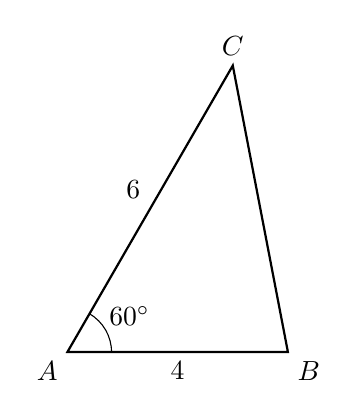
\begin{tikzpicture}[scale=0.7]
			\coordinate (A) at (0,0);
			\coordinate (B) at (4,0);
			\coordinate (C) at (3,{6*sin(60)});
			\draw[thick] (A) -- (B) -- (C) -- cycle;
			\draw (0.8,0) arc[start angle=0,end angle=60,radius=0.8];
			\node at (30:1.3) {$60^\circ$};
			\node[below left] at (A) {$A$};
			\node[below right] at (B) {$B$};
			\node[above] at (C) {$C$};
			\node[below] at (2,0) {$4$};
			\node[above left] at (1.5,2.6) {$6$};
		\end{tikzpicture}
	\end{center}

	\begin{correction}
		D'après le théorème d'Al Kashi :
		\[
			\begin{array}{rrcll}
				     & BC^2 & = & AB^2 + AC^2 - 2 \times AB \times AC \times \cos\pa{\widehat{BAC}} &                                 \\
				\iff & BC^2 & = & 4^2 + 6^2 - 2 \times 4 \times 6 \times \cos 60^\circ              &                                 \\
				\iff & BC^2 & = & 16 + 36 - 48 \times \tfrac{1}{2}                                  &                                 \\
				\iff & BC^2 & = & 28                                                                & \iff BC=\sqrt{28} \approx 5{,}3
			\end{array}
		\]

	\end{correction}
\end{methode}

\begin{methode}[Appliquer le théorème d'Al Kashi pour calculer un angle]
	On considère la figure ci-dessous. Calculer la mesure de l'angle $\widehat{BAC}$ arrondie au degré près.

	\begin{center}
		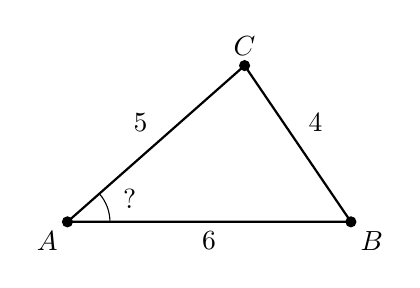
\begin{tikzpicture}[scale=0.6]
			\coordinate (A) at (0,0);
			\coordinate (B) at (6,0);
			\coordinate (C) at (3.75,{sqrt(10.9375)});
			\draw[thick] (A) -- (B) -- (C) -- cycle;
			\draw (0.9,0) arc[start angle=0,end angle=41.41,radius=0.9];
			\node at (20:1.4) {$?$};
			\node[below left] at (A) {$A$};
			\node[below right] at (B) {$B$};
			\node[above] at (C) {$C$};
			\node[below] at (3,0) {$6$};
			\node[above left] at (1.9,1.7) {$5$};
			\node[above right] at (4.9,1.7) {$4$};
			\foreach \pt in {A, B, C}{ \filldraw (\pt) circle (3pt); }
		\end{tikzpicture}
	\end{center}

	\begin{correction}
		D'après le théorème d'Al Kashi :
		\[
			\def\arraystretch{1.4}
			\begin{array}{rccccccl}
				     & BC^2                     & = & AB^2                       & +       & AC^2         & - & 2 \times AB \times AC \times \cos\pa{\widehat{BAC}} \\
				\iff & 4^2                      & = & 6^2                        & +       & 5^2          & - & 2 \times 6 \times 5 \times \cos\pa{\widehat{BAC}}   \\
				\iff & 16                       & = & 36                         & +       & 25           & - & 60\cos\pa{\widehat{BAC}}                            \\
				\iff & 60\cos\pa{\widehat{BAC}} & = & 36                         & +       & 25           & - & 16 \quad= 45                                        \\
				\iff & \cos\pa{\widehat{BAC}}   & = & \tfrac{45}{60}             & =       & \tfrac{3}{4} &   &                                                     \\
				\iff & \widehat{BAC}            & = & \cos^{-1}\pa{\tfrac{3}{4}} & \approx & 41^\circ     &   &
			\end{array}
		\]

	\end{correction}
\end{methode}

\section{Application à la physique : le travail d'une force}

\begin{defin}
	Le \textbf{travail} $W$ d'une force constante $\vec{F}$ lors d'un déplacement $\vec{\ell}$ mesure la participation de cette force dans le déplacement d'un mobile.

	Il est défini comme le produit scalaire du vecteur force par le vecteur déplacement :
	\[
		W = \vec{F}\cdot\vec{\ell}
	\]

	Il se mesure en joules (J).
\end{defin}

\begin{ex}
	Une dépanneuse remorque une voiture en panne sur une côte.

	La tension du câble est constante et égale à $1600$ N.

	Le câble fait un angle de $30^\circ$ avec le plan de la route et la voiture est remorquée sur une distance de $500$ m.

	Quel est le travail effectué par la dépanneuse sur la voiture ?

	\begin{center}
		\begin{tikzpicture}[scale=1.1]
			\draw[->,very thick,bleu] (0,0) -- (5,0) node[midway,below] {$\vec{\ell}$};
			\draw[->,very thick,rouge] (0,0) -- (30:3.2) node[above right] {$\vec{F_T}$};
			\draw[dashed,gris] (30:3.2) -- ({3.2*cos(30)},0);
			\draw[->] (0.9,0) arc[start angle=0,end angle=30,radius=0.9];
			\node at (15:1.3) {$30^\circ$};
		\end{tikzpicture}
	\end{center}

	L'angle de la route n'a pas d'importance : l'angle entre la force $\vec{F_T}$ et le déplacement $\vec{\ell}$ est de $30^\circ$.

	On a :
	\[
		\def\arraystretch{1.4}
		\begin{array}{rcl}
			W & = & \vec{F_T}\cdot\vec{\ell}                                      \\
			  & = & F_T \times \ell \times \cos 30^\circ                          \\
			  & = & 1600 \times 500 \times \dfrac{\sqrt{3}}{2}                    \\
			  & = & 400\,000\sqrt{3}\,\text{ J} \quad \approx 692{,}82 \text{ kJ}
		\end{array}
	\]

\end{ex}

% \section{Exercices}
%
% \begin{exo}
% 	Soit $ABC$ un triangle équilatéral de côté $4$. Calculer les produits scalaires $\vec{AB}\cdot\vec{AC}$, $\vec{BA}\cdot\vec{BC}$ et $\vec{AB}\cdot\vec{BC}$.
% \end{exo}
%
% \begin{exo}
% 	Soit $\vec{u}$ et $\vec{v}$ deux vecteurs de normes respectives $3$ et $2$ et tels que $\vec{u}\cdot\vec{v} = -2$. Calculer :
% 	\[
% 		\pa{\vec{u} + \vec{v}}^2 \quad;\quad \pa{\vec{u} - \vec{v}}^2 \quad;\quad \pa{2\vec{u} + \vec{v}}\cdot\pa{\vec{u} - 3\vec{v}}
% 	\]
%
% \end{exo}
%
% \begin{exo}
% 	Soit $ABCD$ un carré de côté $5$. Calculer les produits scalaires :
% 	\[
% 		\vec{AB}\cdot\vec{AC} \quad;\quad \vec{AB}\cdot\vec{AD} \quad;\quad \vec{AD}\cdot\vec{CB} \quad;\quad \vec{AB}\cdot\vec{CD}
% 	\]
%
% \end{exo}
%
% \begin{exo}
% 	Soit $ABCD$ un parallélogramme tel que $AB = 5$, $AD = 3$ et $AC = 7$. Calculer le produit scalaire $\vec{AB}\cdot\vec{AD}$.
% \end{exo}
%
% \begin{exo}
% 	Le plan est muni d'un repère orthonormé $\vOIJ$.
% 	\begin{enumerate}
% 		\item Soit $\vec{u}\coord{3}{-2}$ et $\vec{v}\coord{4}{6}$. Calculer $\vec{u}\cdot\vec{v}$ et $\norm{\vec{u}}^2$. Que peut-on dire des vecteurs $\vec{u}$ et $\vec{v}$ ?
% 		\item On considère les points $A\coordl{0}{1}$, $B\coordl{4}{3}$ et $C\coordl{-1}{3}$. Démontrer que le triangle $ABC$ est rectangle en $A$.
% 		\item On considère les points $A\coordl{-1}{1}$, $B\coordl{2}{3}$ et $C\coordl{3}{-1}$. Calculer une valeur approchée au degré près de l'angle $\widehat{BAC}$.
% 	\end{enumerate}
% \end{exo}
%
% \begin{exo}
% 	\nline
% 	\begin{enumerate}
% 		\item Dans un triangle $ABC$, on a $AB = 7$, $AC = 5$ et $\widehat{BAC} = 60^\circ$. Calculer $BC$ (valeur arrondie au dixième).
% 		\item Dans un triangle $ABC$, on a $AB = 7$, $AC = 5$ et $BC = 8$. Calculer la mesure de l'angle $\widehat{BAC}$ arrondie au degré près.
% 	\end{enumerate}
% \end{exo}
%
% \begin{exo}
% 	Une force constante de $200$ N fait un angle de $40^\circ$ avec le déplacement de son point d'application. Calculer, en joules et arrondi à l'unité, le travail de cette force lors d'un déplacement de $30$ m.
% \end{exo}
